\documentclass[10pt, a4paper]{article}
\usepackage{cmap}
\usepackage[T2A]{fontenc}
\usepackage[utf8]{inputenc}
\usepackage[english, russian]{babel}
\usepackage[dvipsnames,table,xcdraw]{xcolor}
\usepackage{
	amsmath,
	amssymb,
	scrextend,
	enumitem,
	pscyr,
	multicol,
	cmap,
	titling,
	indentfirst,
	cancel,
	wrapfig,
	gensymb,
	tikz,
	graphicx,
	fancyhdr,
	mathrsfs,
	graphbox,
	indentfirst
}
%Параметры страницы
\usepackage[left=15mm,right=15mm,
top=2cm,bottom=2cm]{geometry}
\pagestyle{fancy}
%Путь к картинкам
\graphicspath{{pic/}}
\DeclareGraphicsExtensions{.pdf,.png,.jpg}
%Числа в списке второго уровня по умолчанию
\renewcommand{\labelenumii}{\arabic{enumii})}
%Новые команды
\definecolor{silver}{rgb}{0.7, 0.7, 0.7}
\definecolor{dark}{rgb}{0.3, 0.3, 0.3}
\definecolor{harvestgold}{rgb}{0.85, 0.57, 0.0}
\newcommand{\answer}[1]{\textcolor{silver}{\fbox{#1}}}
\newcommand{\ranswer}[1]{\textcolor{silver}{\begin{flushright}\vspace{-1em}\fbox{#1}\end{flushright}}}
\newcommand{\leveli}{\textcolor{dark}{$\blacksquare\square\square$}\hspace{0.5em}}
\newcommand{\levelii}{\textcolor{dark}{$\blacksquare\blacksquare\square$}\hspace{0.5em}}
\newcommand{\leveliii}{\textcolor{dark}{$\blacksquare\blacksquare\blacksquare$}\hspace{0.5em}}

%Русские символы в списке
\AddEnumerateCounter{\asbuk}{\russian@alph}{щ}

%Сеттеры
\setlength{\parindent}{5ex}
\setlength{\parskip}{1em}

\begin{document}

\lhead{Группа 82}
\chead{Модуль 5 Урок 7}
\rhead{Школа <<Симметрия>>}

\begin{enumerate}
	\item Принадлежит ли точка с координатами $(-5;-2)$ уравнению прямой $y=0,75x+3$?
	\item Принадлежит ли точка с координатами $(-3;-8)$ уравнению прямой $y=2x-2$?
	\item Выяснить, лежат ли точки $A(6;-6)$, $B(10;10)$ и $C(12;18)$ на одной прямой.
	\item Найдите координаты точки пересечения пересечения прямых $y=\dfrac{1}{2}x$ и $y=x+4$.
	\item Найдите координаты точки пересечения пересечения прямых $y=3x-5$ и $y=\dfrac{3}{5}x+7$.
	\item Выяснить, можно ли через точки $A(-6;-2)$, $B(8;6)$, $C(-8;-8)$ и $D(8;-4)$ провести две параллельные прямые.
	\item Найдите уравнение прямой, которая проходит через точку $(3;-1)$ и параллельна прямой $y=\dfrac{1}{5}x+4$.
	\item Найдите уравнение прямой, которая проходит через точку $(6;0)$ и перпендикулярна прямой $y=-0,5x-0,5$.
	\item Найдите координаты точки пересечения двух перпендикулярных прямых, если известно, что первая прямая задана уравнением $y=-0,25x-1,5$, а вторая проходит через точку $(6,5;1)$.
	\item Известно, что точки $A(10;-4)$, $B(4;2)$ и $C(8;6)$, а $ABCD$ --- прямоугольник. Найдите координаты точки $D$.
	\item
	\begin{minipage}[t]{0.6\textwidth}
		 Прямые $f(x)=x-5,5$ и $g(x)$ пересекаются в точке с координатами $(a;b)$. Найдите $a+b$.
	\end{minipage}
	\begin{minipage}[t]{0.3\textwidth}
		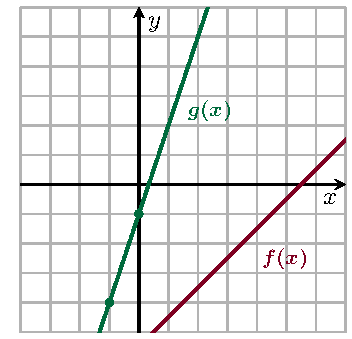
\includegraphics[align=t, width=\textwidth]{graph_6}
	\end{minipage}
\end{enumerate}
\end{document}